\documentclass{report}
\usepackage[utf8]{inputenc}

\usepackage{graphicx}
\usepackage{float}
\usepackage{subcaption}
\usepackage{changepage}
\usepackage[ruled,vlined]{algorithm2e}
\usepackage{url}

\usepackage{geometry}
\geometry{margin=1.7in}
\usepackage[nottoc,numbib]{tocbibind}
\usepackage[export]{adjustbox}[2011/08/13]
\usepackage{hyperref}
\usepackage{xcolor}
\hypersetup{
	colorlinks,
	linkcolor={blue!50!black},
	citecolor={blue!50!black},
	urlcolor={blue!80!black}
}

%\usepackage{chngpage}


\usepackage[labelfont=bf, tableposition=top]{caption}

\usepackage{float}
\floatstyle{plaintop}
\restylefloat{table}

\begin{document}

\title{Leveraging Image Retrieval for Unsupervised Detection of Recurring Content in TV Shows\'{} Video Files}
\author{Master\'{}s Thesis\\ \\ Niels ten Boom \\ [1cm]{\small \textbf{Supervisor:} Prof. dr. ir. A.P. de Vries} \\ {\small \textbf{Second reader:} Prof. M.A. Larson \,\,\,\,\,\,\,\,} \\ {\small \textbf{\,External supervisor (RTL):} D. Odijk}}

\date{\vspace{-3ex}}

\maketitle
\newpage

\begin{abstract}
This thesis presents research on image retrieval-based approaches for recurring content detection in Video On Demand (VOD) TV-shows. The method utilizes feature vectors constructed from video frames and an image retrieval framework to efficiently compare frame similarity across TV-show episodes, these frame similarities are then used to detect recurring parts. A best precision score of 0.884 at 0.687 recall and a best recall score of 0.892 at 0.748 precision were achieved. An altered experimental setup for bumper detection achieved a best precision score of 0.611 at 0.917 recall and a best recall score of 0.979 at 0.288 precision. With these results we present novel research for unsupervised detection of recurring content in VOD shows.
\end{abstract}
\newpage

\tableofcontents
\newpage

\chapter{Introduction} \label{introduction}
Viewing rates for TV are dropping gradually while the number of users of streaming services such as Netflix and Videoland are growing rapidly year over year. This shift from TV to Video on Demand introduces new problems for broadcasters, as they now have to support a hybrid form of traditional broadcasting and Video On Demand (VOD). In this thesis we consider a method that could help to improve the user experience for VOD.

Video content is optimized for just one form, and currently that is broadcast television. This means that the video content may contain recurring content consisting of: recaps, opening credits, bumpers (to ease a viewer into commercials), closing credits and previews. A viewer watching this content back-to-back may find it preferable to be able to skip this recurring content to improve their viewing experience. Providing this functionality to users, requires metadata on where the skippable content occurs in the videos. For a large percentage of content, such metadata has not been retained. Videoland currently hosts over 1000 different titles consisting of multiple seasons and episodes and this selection is always changing. An automated solution that can detect this content in videos would be very useful to transform the video content into a format suited for VOD. In this thesis we will explore methods for such an automated solution.

There is little margin for error with this solution. The accuracy of the end result should be sufficiently high for it to be trusted to label all of the content automatically. If that is not the case, it needs double checking by a human, because if a part of the video gets mislabeled, a user may skip over actual content. It is critical to RTL that this does not happen.

This thesis presents research on unsupervised detection of recaps, opening credits, bumpers, closing credits and previews given the video files from a TV-show. We are going to attempt to tackle this problem by using image retrieval techniques. The motivation behind this is that the overlapping characteristic of the segments is that they reoccur. To be able to detect recurring content we are going to compare similarities of frames across content, this should be done efficiently and accurately, both attributes are important in image retrieval research. Our main research question then is:
\newline
\begin{adjustwidth}{0.3in}{0.3in}
\textit{\textbf{How well does an image retrieval approach perform in accurately detecting recurring content across a TV-show?\newline}}
\end{adjustwidth}
With the subquestions: \\
\begin{adjustwidth}{0.3in}{0.3in}
	\textit{\textbf{How can image retrieval be used to detect recurring content?\newline}}\\
	\textit{\textbf{How accurate is each image retrieval approach?\newline}}\\
	\textit{\textbf{How can the best method be utilized in practice?\newline}}
\end{adjustwidth}
This thesis aims to answer aforementioned research questions. Our hypothesis is that such a method may achieve a level of effectiveness that allows practical application at RTL. The rest of this chapter will be used to expand on the different type of video classes which this research is focused on. Chapter \ref{relatedwork} discusses related work. Chapter \ref{section:imageretrieval} elaborates on the used methods for image retrieval. Chapter \ref{methodology} describes the data and methodology and then the produced results are presented in Chapter \ref{results}. Lastly, the results are discussed in Chapter \ref{discussion} and a conclusion is drawn in Chapter \ref{conclusion}.

\section{Recurring Content Classes} \label{section:segmentclasses}
In this section we discuss the different types of content to be detected. What all the content classes have in common is that they (partially) reappear in previous or future episodes or, as is the case with bumpers; that the content reappears within the episode itself. We will use this attribute for the detection.

\subsubsection{Recaps}
A television show typically has recaps before the opening credits. In the recaps content of previous episodes is repeated to refresh the viewer's memory. This is useful for linear TV when an episode is aired every week. Someone watching episodes back-to-back ideally wants to skip the recaps together with the opening credits because they have seen the content recently. Not all material preceding the opening credits is a recap though, it can be original content. See Figure \ref{fig:contextrecaps} for a visual example.

\begin{figure}[H]
	\makebox[\textwidth][c]{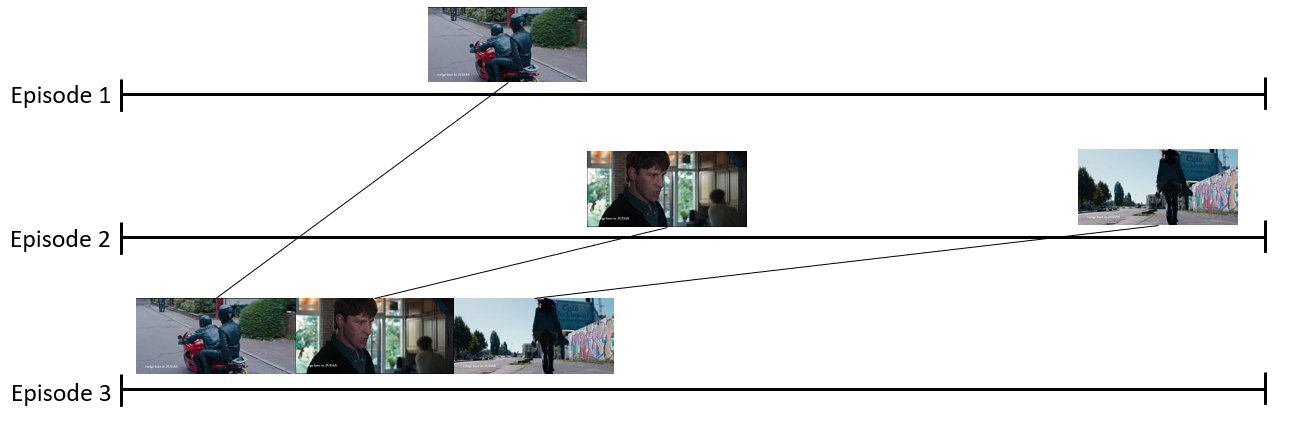
\includegraphics[width=\paperwidth,center, scale=0.8]{images/context_recaps.png}}
	\caption{\textbf{Visual depiction of recaps. Shots from episode 1 and 2 are shown at the start of episode 3 to give a brief summary of important events.}}
	\label{fig:contextrecaps}
\end{figure}

\subsubsection{Opening credits}
The opening credits of a TV-show are generally the same for all of the episodes in the same season. It typically opens the show with a theme song, presenting the most important actors at the start. There is no prior knowledge on how the opening credits of a show look like and they often change every season, therefore the detection should be unsupervised. See Figure \ref{fig:contextopeningcredits} for a visual example.

\begin{figure}[H]
	\makebox[\textwidth][c]{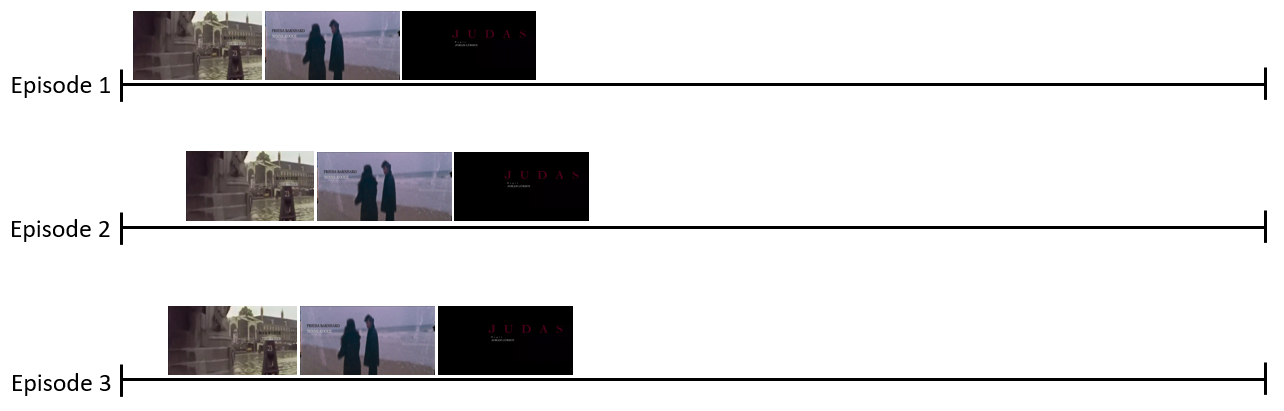
\includegraphics[width=\paperwidth,center, scale=0.8]{images/context_openingcredits.png}}
	\caption{\textbf{Visual depiction of opening credits. A very similar sequence of shots that start at different times at the beginning of an episode.}}
	\label{fig:contextopeningcredits}
\end{figure}

\subsubsection{Bumpers}
The bumper is a part of the video that eases a viewer into the upcoming commercial. Most of the times it has a voice over and text on screen saying: 'Next' (or the dutch translation of 'next') and footage of what is to be expected after the commercial break is shown. See Figure \ref{fig:contextbumpers} for a visual example.

\begin{figure}[H]
	\makebox[\textwidth][c]{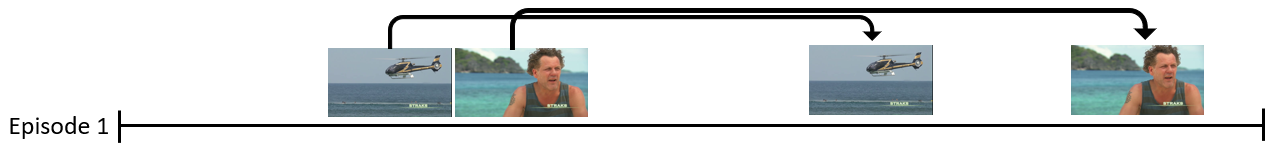
\includegraphics[width=\paperwidth,center, scale=0.8]{images/context_bumpers.png}}
	\caption{\textbf{Visual depiction of bumpers. A summary of important shots are shown together that will occur at a later point of time in the episode.}}
	\label{fig:contextbumpers}
\end{figure}

\subsubsection{Previews}
A preview is a segment at the end of an episode playing an advance showing of fragments of the next episode(s) are played. Previews can typically be found in content that was created specially for broadcast TV. It gives the viewer a taste of what to expect in the next episode that will air a week later. These previews may contain overlayed credits of people who helped in the production of the show. See Figure \ref{fig:contextpreviews} for a visual example.

\begin{figure}[H]
	\makebox[\textwidth][c]{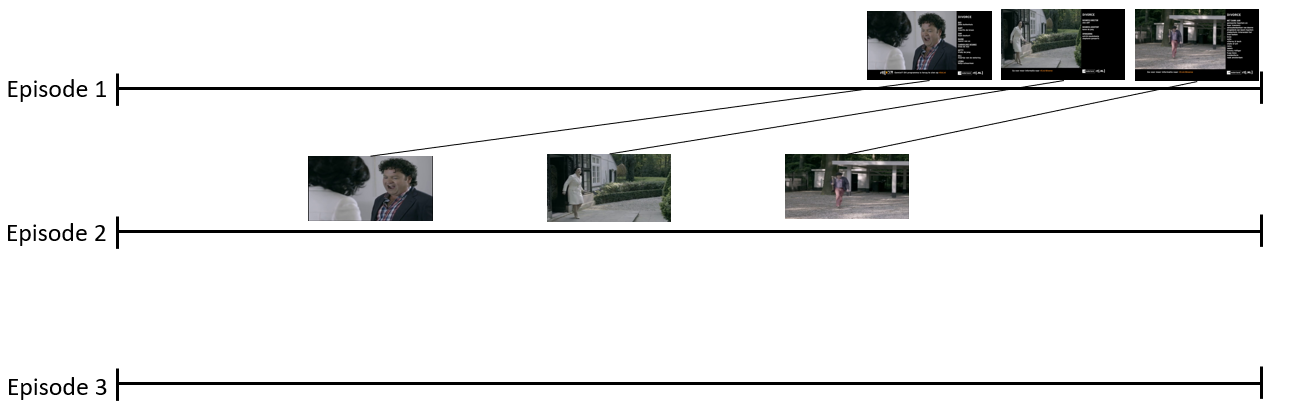
\includegraphics[width=\paperwidth,center, scale=0.8]{images/context_previews.png}}
	\caption{\textbf{Visual depiction of previews. It shows shots that will occur in the next episode with a textual overlay.}}
	\label{fig:contextpreviews}
\end{figure}

\subsubsection{Closing Credits}
The closing credits at the end of a video mostly consist of scrolling text and there is little variation between the frames. In these texts everybody related to the production of the video is mentioned. In general the frames all have a black background with white text. But backgrounds can also vary, therefore a solution that simply looks for black and white would not suffice. See Figure \ref{fig:contextclosingcredits} for a visual example.

\begin{figure}[H]
	\makebox[\textwidth][c]{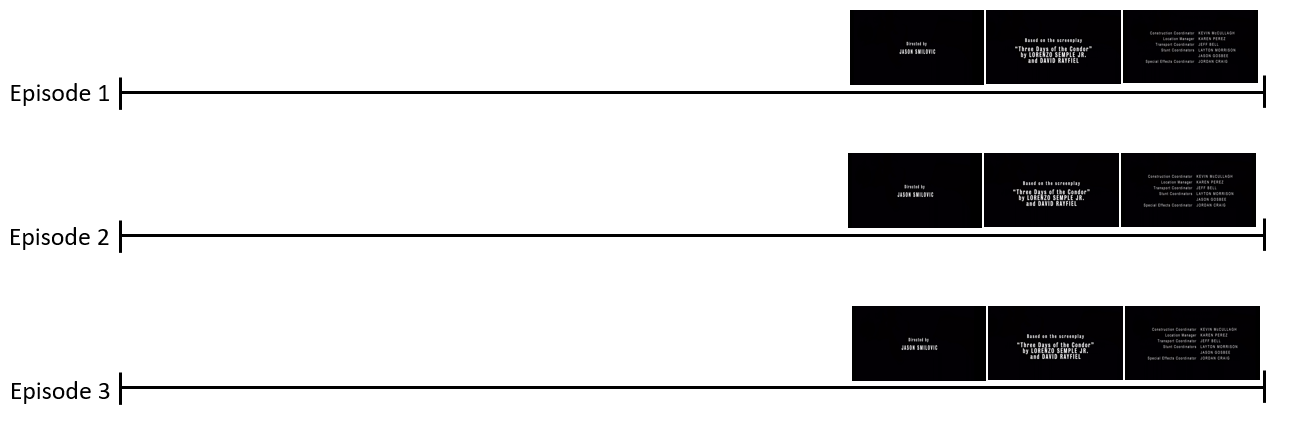
\includegraphics[width=\paperwidth,center, scale=0.8]{images/context_closingcredits.png}}
	\caption{\textbf{Visual depiction of closing credits. Frames consisting of text at the end of each episode in which the actors, producers and others related to the show are given credit.}}
	\label{fig:contextclosingcredits}
\end{figure}

\section{Definitions}
This section will be used to introduce definitions used throughout this thesis. We define a season with multiple episodes of a TV-show as T.
\[T = \{E_1, E_2, \dots, E_x\}\]
An episode within a season is defined as a set of frames.
\[E = \{f_1, f_2, \dots, f_y\}\]
The videos contains shot boundaries, we refer the set of locations of shotboundaries as B.
\[B = \{b_1, b_2, \dots, b_z\}\]

\chapter{Related Work} \label{relatedwork}

No prior work exists that explores a solution for the problem previously described (unsupervised detection of these specific recurring segments). Related work exists that focuses on commercial or repeated sequence detection in large broadcast streams. These detection methods can be roughly divided into three groups: fingerprint, feature-based and unsupervised methods. 

%fingerprint
Fingerprint methods set up a database of fingerprints of known commercials or repeated sequences to detect these in a broadcast stream. Lienhart et al.\ \cite{lienhart1997detection} propose a method based on features to roughly localize advertisements in a stream and then construct a fingerprint database based on color coherence vectors. Gauch et al.\ \cite{gauch2006finding} propose a method based on constructing feature vectors from color moments in a stream. Covell et al.\ \cite{covell2006advertisement} implement a fingerprinting method based on audio with visual verification after a proposed match. The disadvantage of these fingerprinting methods is that it is not unsupervised and the setting up and maintenance of such a fingerprint database requires much work.

%fingerprint methodes geven vaak ook methode voor repeated sequence detection maar met onvoldoende precisie

%feature based
Feature-based methods detect commercials based on extracted video features. Wang et al.\ \cite{wang2008multimodal} fuse the results of audio scene changes and textual content similarity between shots to segment programs including commercials.

%clustering
With the unsupervised methods the authors typically do a dimensionality reduction operation and then try to find repeated sequences or commercials with clustering methods. Herley et al.\ \cite{herley2006argos} convert the stream with a Discrete Cosine Transform (DCT) to reduce dimensionality and then propose an extensive probability framework to detect repeated sequences. Benezeth et al.\ \cite{benezeth2010unsupervised} use the Electronic Programme Guide (EPG) in addition to the dimensionality reduction to detect program boundaries.

%vergelijkbare dingen
Abduraman et al.\ \cite{abduraman2011unsupervised} propose a system to detect repeated sequences in streams by performing a DCT operation on all of the frames in the stream and then use a micro clustering technique to detect repeated sequences. They were also able to link the trailers to their respective programs that occur at a later point in the stream.

All of the previously mentioned works never cover the specific topic of segmenting the classes mentioned in Section \ref{section:segmentclasses} and use properties only available to broadcast streams such as the EPG. The methods also focused on recurring content detection are exclusively based on detection of moderate to long sequences, it does not cover short recurring sequences stitched together such as a recap. The methods yielded high accuracies in the range of 90\% - 95\% precision, also most research is from many years ago and work that focuses on repeated sequence detection in broadcast streams do not vary much in methodology. This work is not focused on broadcast streams and aims for higher accuracies, we will not replicate the previously mentioned methodologies, however from the aforementioned papers we conclude that a large dimensionality reduction step will be necessary to efficiently process a large visual data set.
\\

Dimensionality reduction and efficient matching of large amounts of visual data is important within content based image retrieval, Zheng et al. give a detailed summary of the most significant contributions from past years \cite{zheng2018sift}. Their summary covers three periods in image retrieval: Early methods, SIFT-based methods and Convolutional Neural Network (CNN) based methods. Smeulders et al. present all the contributions of the early methods \cite{smeulders2000content}, these methods focused on looking at the color, texture and local geometry of images for retrieval \cite{yu2002color,manjunath1996texture}. Not much later the Bag-of-words (BoW) model was proposed as a new method for image retrieval \cite{sivic2003video}. The advantage of this is that inverted indexes can be used for immediate retrieval of similar images. The BoW model paired with SIFT-descriptors \cite{lowe2004distinctive} as the feature vectors was used in image retrieval research for years \cite{nister2006scalable,philbin2007object,jegou2008hamming,jegou2010aggregating,jegou2012aggregating}. Since 2012 when the convolutional neural network was introduced \cite{krizhevsky2012imagenet} research switched to CNN-based methods for image retrieval because they achieved better performance on a variety of image retrieval tasks	 \cite{babenko2014neural,yue2015exploiting, tolias2015particular}.

\section{Shot Change Detection}

Shot detection is a technique that can be used on videos to determine shot boundaries, see Figure \ref{shotchange} for an example of such a shot change. 

\begin{figure}[H]
	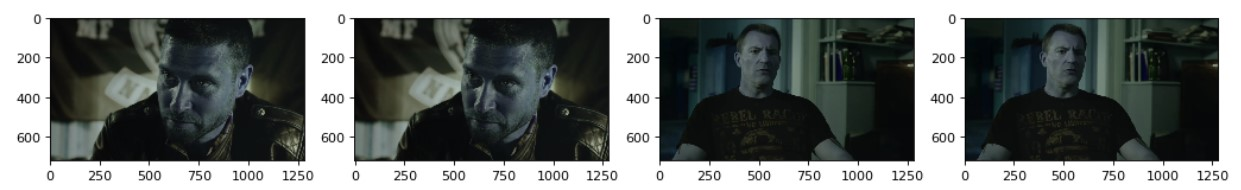
\includegraphics[width=12cm]{images/shotchange.jpg}
	\centering
	\caption{\textbf{Example of a shot change within 4 frames of a video.}}
	\label{shotchange}
\end{figure}

Shot detection is going to be used and thus will we expand on it. A lot of research has been done related to shot detection \cite{lienhart1998comparison} and many techniques have been proposed. 

We use a method that looks at the shift in mean color in HSV space \cite{shao2015shot}. The shot boundaries are classified by calculating the difference in hue, saturation and value for each frame and then from this the mean is calculated. If the mean is higher than a threshold H, then a shot boundary is marked, refer to algorithm \ref{algorithm:shotboundary} for a pseudo-code representation.

\begin{algorithm}[H] 
	\SetAlgoLined
	shotBoundaries = List()\;
	previousMeanHSV = getMeanHSV(Episode[0])\;
	\For{frame in Episode}{
		meanHSV = getMeanHSV(frame)\;
		\If{abs(meanHSV - previousMeanHSV) $>$ H}{
			shotBoundaries.add(frame)\;
		}
		previousMeanHSV = meanHSV\;
	}
	\caption{\textbf{Shot boundary detection}}
	\label{algorithm:shotboundary}
\end{algorithm}


\iffalse
%oude paper OCR op video
\cite{li2000automatic} %TODO

%fingerprints
\cite{lienhart1997detection} %commercial detection met fingerprints
\cite{covell2006advertisement} %commercial detection fingerprints

%features
\cite{gauch2006finding} %commercial detection features
\cite{wang2008multimodal} %doen programma segmentatie

%clustering
\cite{herley2006argos} %argos paper gebruikt audio en heel veel probability
\cite{berrani2008non} %micro clustering repeated sequence detection

\cite{benezeth2010unsupervised} %enige paper die iets vergelijkbaars doet, maar op basis van stream en programmagids, veel nuttige references
\cite{ibrahim2011tv} %andere vergelijkbare paper, op advertenties en met grote stream
\cite{abduraman2011unsupervised} %Ook hele vergelijkbare paper, werken ook weer met DCT en KVD maar recall en precision round 0.95
\fi


\chapter{Image Retrieval} \label{section:imageretrieval}
Image retrieval is a subset of the research field Information Retrieval (IR). It investigates the problem where one has a query \textbf{q} expressing an information need and wants to find the best possible match for this \textbf{q} in a set of documents \textbf{D}.

In the case of image retrieval the query consists of an image for which the best matching image should be found in a document set of images. There are two approaches for doing this.

\begin{figure}[H]
	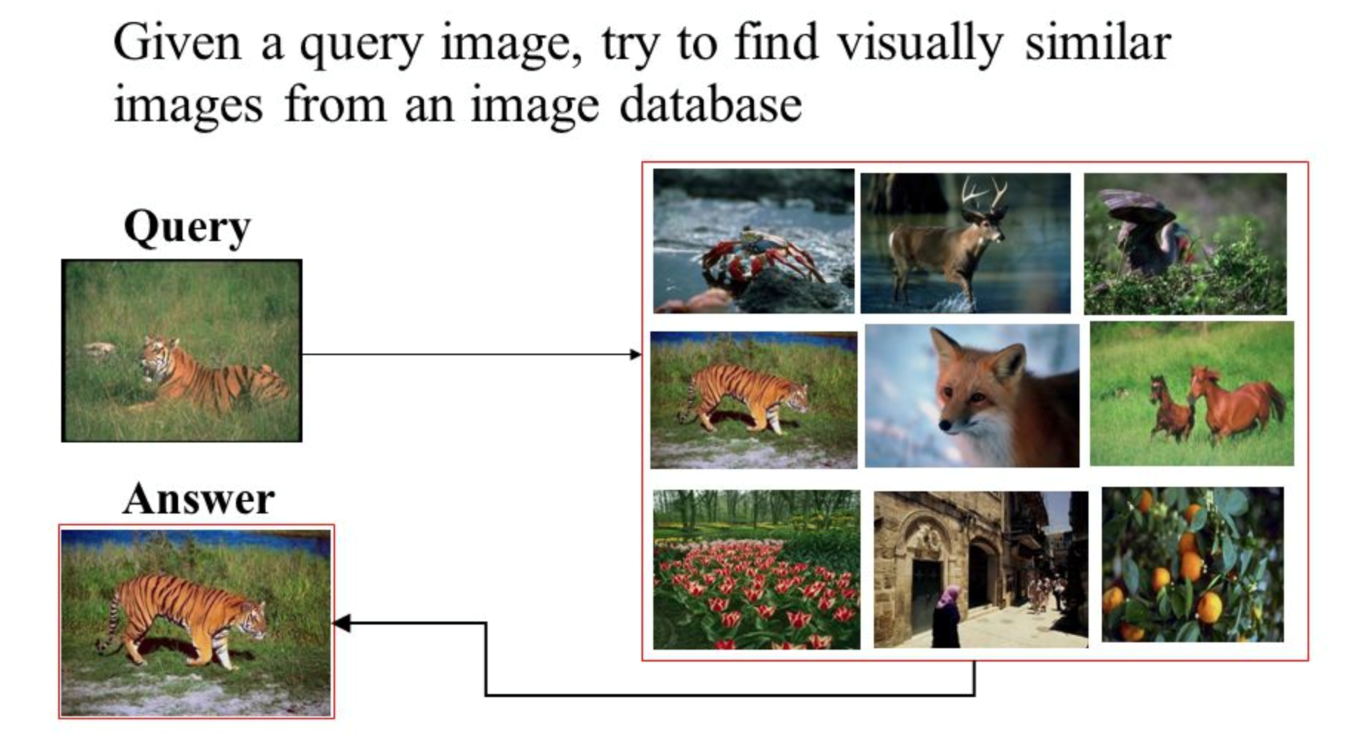
\includegraphics[width=8cm]{images/imageretrieval.png}
	\centering
	\caption{\textbf{Visual example of image retrieval.}}
	\label{fig:imageretrieval}
\end{figure}

\textbf{Text-based image retrieval} refers to retrieval of images based on textual metadata associated with these images. It matches images based on their titles, keywords and more. The downside of this method is that if there is no metadata available then it needs to be added manually. With the growing sizes of image databases this can become quite inefficient, hence the more focus on content-based image retrieval in past years \cite{rajam2013survey}.

\textbf{Content-based image retrieval} is retrieval based on the content of the image rather than the metadata as is the case with concept-based image retrieval. Computer vision is used to evaluate the image similarity, this can be done by looking at colors, shapes, textures and more. The advantage of content based image retrieval is that it does not rely on the metadata of images and thus does not require manual labeling.

\section{Feature vectors}
A feature vector is a vector containing a numeric representation of multiple characteristics of an object. In this case the objects are images, the frames of a video. To illustrate feature vectors for images, a small example is given. Consider the following three images of 10 by 10 pixels consisting only of black or white pixels in Figure \ref{featurevectorimages}.

If we would like to measure the image similarity between these pictures then we could do this on a pixel-per-pixel basis, while this could work for low dimensional images, comparing HD images consisting of 1920 pixels by 1080 pixels would require massive computation and will require extensive logic to handle small deviations between images. This can be resolved by creating feature vectors to represent the images. A representation for these example images could be the number of black and white pixels in the image, resulting in the feature vector; $\textbf{x} = [\#\;white\;pixels, \#\;black\;pixels]^T$. This vector can now be represented in 2D-space, and compared to other vectors in 2D space by calculating the distance between other points in that space. The distance could for example be computed by calculating the euclidean distance between each vector.

\[d(\textbf{p,q}) = \sqrt{(p_1 - q_1)^2 + \dots + (p_n - q_n)^2} \]

\begin{figure}[H]
	\centering
	\begin{subfigure}[b]{0.2\textwidth}
		
\includegraphics[width=\textwidth]{images/mostlywhite.png}
	\end{subfigure}\hfill
	\begin{subfigure}[b]{0.2\textwidth}
		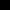
\includegraphics[width=\textwidth]{images/allblack.png}
	\end{subfigure}\hfill
	\begin{subfigure}[b]{0.2\textwidth}
		
\includegraphics[width=\textwidth]{images/mostlyblack.png}
	\end{subfigure}
	\caption{Three images of 10x10 pixels, consisting of only black and white pixels. The resulting feature vectors are $[64,36]^T$, $[0, 100]^T$ and $[25,75]^T$ respectively.}
	\label{featurevectorimages}
\end{figure}

Figure \ref{fig:distanceexample} plots the feature vectors and the distances between. Example images 2 and 3 are the most alike because the distance between them is the smallest. Which seems in line with a visual inspection.

\begin{figure}[H]
	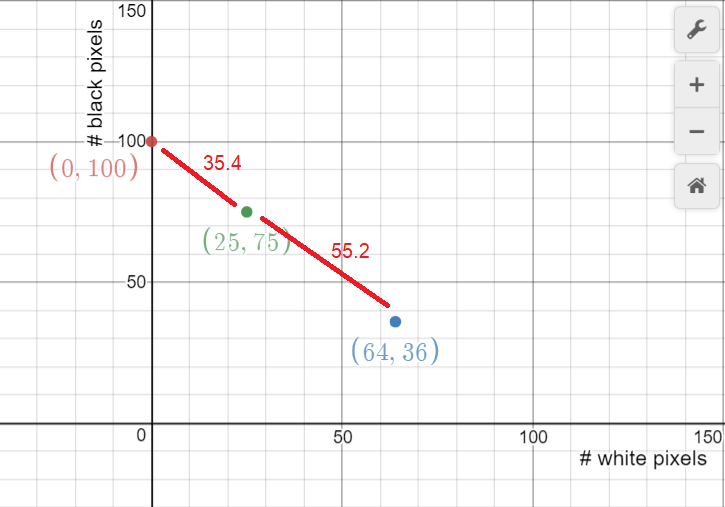
\includegraphics[width=8cm]{images/distanceexample.png}
	\centering
	\caption{Example of distance in 2D between feature vectors that represent the example images. According to the chosen features, image 2 and 3 are the most alike.}
	\label{fig:distanceexample}
\end{figure}

The similarity of images can be determined by computing the distance between their feature vectors. A low distance indicates a higher similarity. Counting the number of black and white pixels for the construction of feature vectors is not a very robust method, a lot of research in image retrieval focused on the construction of alternative feature vectors to achieve better retrieval results most in line with human judgment. Part of this thesis is determining the best method for the construction of the image feature vectors to apply for our problem. We will expand on the methods that are going to be explored. 

%Misschien uitwijden over local en global descriptors
As mentioned in Chapter \ref{relatedwork}, Zheng et al. \cite{zheng2018sift} outline three significant periods in image retrieval, the early methods focused on global descriptors mostly based on color and texture. These global descriptors were not good at handling image changes in illumination, translation, occlusion and truncation. This gave rise to local descriptors based SIFT methods until recently CNN-descriptors became the most popular. 

We want to determine whether global or local descriptors are needed. Therefore we take two different global descriptor methods and one recent local descriptor method with one of the best performances. The chosen methods are color histograms as a global descriptor, color texture moments \cite{yu2002colortexturemoments} as a method that combines the color and texture of an image and lastly CNN-descriptors were implemented as local descriptors.

This is not an exhaustive list of methods, but because computing feature vectors for a large amount of frames is resource intensive, we limited ourselves to these three. If one of the methods achieves promising results then future research can expand on variations of the method or if none of the methods achieve acceptable results, then future research could try other distinct methods.

\section{Color Histograms}
A color histogram is a representation of the distribution of colors in an image. Color histograms are a flexible and low dimensional way of representing images. A color histogram can be computed by counting the number of pixels in a certain color range, the size of this range is variable, called the bin size. A larger bin size results in lower dimensions of the resulting histogram. For example, if one chooses a bin size that is half of the intensity range. The resulting vector would have 6 dimensions, two bins for each color channel. See Figure \ref{fig:colorhistogram} for an example color histogram with such a bin size.
\begin{figure}[H]
	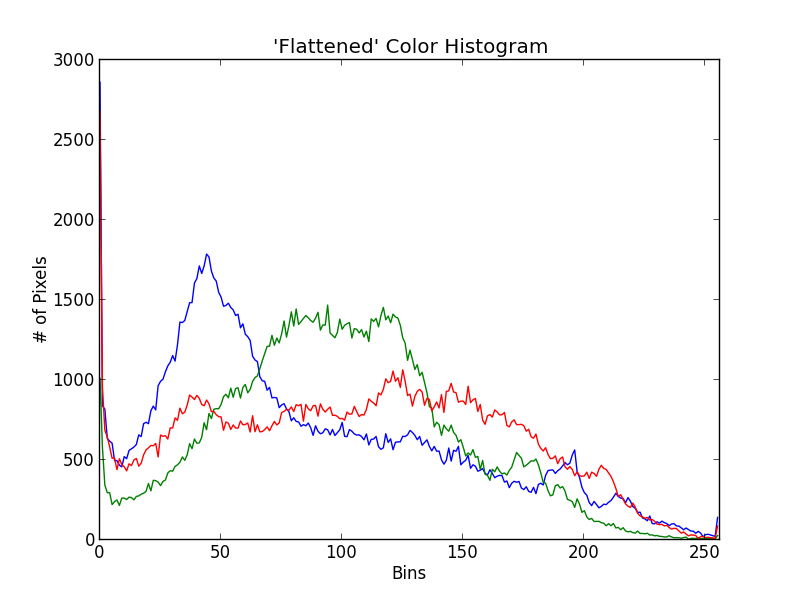
\includegraphics[width=8cm]{images/colorhistogram.png}
	\centering
	\caption{\textbf{Color histogram with a large binsize (binsize=128) for illustration.}}
	\label{fig:colorhistogram}
\end{figure}
Color histograms are global descriptors because they describe the image on a global level. Viewing a frame as a color histogram loses a lot of detail, but for the specific problem recurring video content, this may be sufficient.

\section{Color Texture Moments}
Color texture moments as proposed by Yu et al. \cite{yu2002colortexturemoments} are a low-level feature descriptor that integrates both color and texture characteristics of an image. An image is converted from RGB to HSV color space, and on each color map a 2d convolution is applied for each 3x3 filter shown in Figure \ref{fig:filters}.

\begin{figure}[H]
	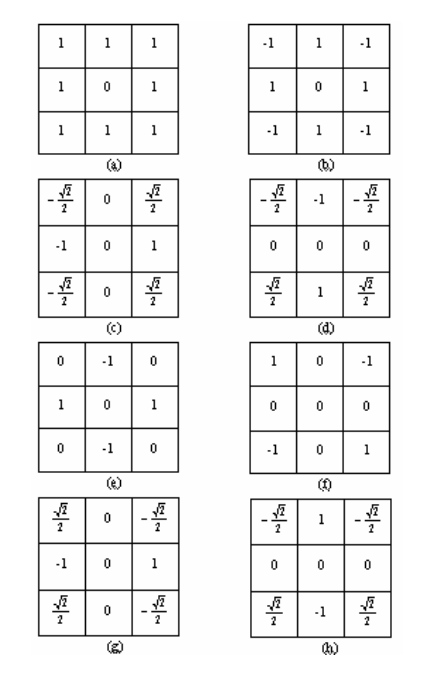
\includegraphics[width=5cm]{images/filters.png}
	\centering
	\caption{\textbf{Filters used for computing the color texture channels.}}
	\label{fig:filters}
\end{figure}

Which results in 8 channels for each color map, 24 channels in total. For each of the resulting channels the first and second color moments, which are the mean and standard deviation, are taken. This results in a 48-dimensional feature vector.

\section{CNN Features} \label{subsection:cnnfeatures}
Convolutional neural networks are very good at image classification and segmentation tasks. However it was found that using the resulting channels after the convolution layers as feature vectors also performs well at image retrieval tasks. There are many ways to construct CNN feature vectors that perform well as described in \cite{zheng2018sift}.

We will use the Regional Maximum Activation of Convolutions (R-MAC) method introduced by Tolias et al. \cite{tolias2015particular} as our implementation for the feature vectors. The frames are fed through a pre-trained VGG16 neural network. The last fully connected layers of the network are discarded, and the resulting channels with activations from the convolutional layers are divided up into regions. For each of these regions the Maximum Activations of Convolutions (MAC) feature vector is calculated, and all these feature vectors are then post-processed by applying L2-normalization, PCA-whitening and L2-normalization. Then all the feature vectors are summed into one resulting feature vector and L2-normalization is applied one last time as the final step, resulting in a 512-dimensional vector. For a more extensive description, one can refer to \cite{tolias2015particular}.

\chapter{Methodology} \label{methodology}
We want to explore whether we can detect recurring content unsupervised and if so, which method of feature vector construction scores the best in terms of precision and recall. Initially a non-generalized approach was tried, where a unique method for each content class was used (For example: OCR for textual closing credits, similarity matrices for opening credits and feature based classification for recaps and previews). However, this was quickly found to be ineffective because of a high variety of edge cases in creative non-structured video content. 

The characteristic of all the segment classes is that they reoccur either in previous or future episodes. To match frames from one episode with other episodes, feature vectors were constructed from the frames and the distances between these vectors were computed and saved. If a part of the video consecutively has matching feature vectors from previous or future episodes, then that part is labeled as a recurring segment. It is therefore important that the resulting feature vectors do not mismatch between actual recurring content and content that looks alike. Methods chosen for construction of the feature vectors should therefore not result in feature vectors of very high dimensionality, because this has proven to reduce the distance between the farthest and closest points \cite{beyer1999nearest}, likely diminishing the distinctive property of the feature vectors that is needed.

We will do separate experiments for the bumper detection as they require a different approach for detection because they only contain recurring content from within an episode itself.

All of the experiments were coded in Python and the code of the experiments can be found on Github \cite{own-github}.
%and executed on AWS m4.2xlarge instances
\section{Data}
The data set contains 80 video files originating from 16 different seasons of tv-shows, amounting to around 50 hours of content. Only for three of these seasons do we use the full array of episodes, from the rest of the seasons, only the first three episodes will be looked at to have a more varied data set at a reasonable amount of human judgement. Originally these files were in \textit{.mxf} full broadcast format, this meant each file being 25GB on average. All the files were converted to MP4 files having a width of 320 pixels width and the length to maintain the aspect ratio. The resizing step was done to drastically decrease the computing time needed. The conversion was done with FFmpeg \cite{ffmpeg}.

For each file the start and end timestamps for the recaps, opening credits, bumpers, closing credits and previews were annotated in HH:MM:SS format in a CSV file, so that it could be loaded and compared effectively.

\begin{table}[h]
	\begin{adjustwidth}{-.5in}{-.5in}  
		\begin{center}
			\begin{tabular}{ l | r c c}
								& Total seconds & \% of recurring 	& \% of total \\
				\hline
				Recaps 			& 3275 			& 34.8\% 			& 1.7\% \\
				Opening credits	& 4669			& 49.5\%			& 2.5\%	\\
				Closing credits	& 690			& 7.3\%				& 0.4\%	\\
				Previews		& 592			& 6.3\%				& 0.3\% \\
				\hline
				Recurring		& 9423			& -					& 4.9\% \\
				\textbf{Total}	& \textbf{188981}		& -					& -
			\end{tabular}
		\end{center}
	\end{adjustwidth}
	\caption{Details of the data that was used to perform the experiments with.}
	\label{table:datastatistics}
\end{table}

Table \ref{table:datastatistics} shows the distribution of the different recurring content classes. It can be noted that the classes are not in balance; the recurring content is weighted towards recaps and opening credits. Recurring content consists of 4.9\% of the total content, thus with a perfect method, that is the percentage of time we could save of people watching the content back-to-back.

\section{Feature Vector Construction}
Video plays at 25 frames per second, and neighboring frames usually vary slightly. We will take advantage of this property to reduce computational complexity, by either sub sampling every 3 frames or only considering shot boundary frames. We take all the video files of a season $E_x \in T$ and convert each file to a set of feature vectors $S_x = \{v_1, v_2, \dots, v_l\}$ with the function $f$.

\[f(E_x) = S_x = \{v_1, v_2, \dots, v_l\}\]

The rest of the sections will expand on different implementations of the function $f$, how the different types of feature vectors are constructed. We use three different methods for the feature vector construction. These methods were chosen because of their efficient computation and accuracy in image retrieval tasks and to see if there is a difference between global and local descriptors applied to this problem. The methods chosen were color histograms, color texture moments and CNN features.

\subsection{Color Histograms}
For the construction of the color histograms the pixel intensities in each channel (Red, Green, Blue (RGB)) are counted and binned according to a specified bin size. All these bins will be concatenated to result in a feature vector, the size of the feature vector is a result of the chosen bin size.

Each single channel is represented by 60 bins. These are then concatenated into a 1D vector, resulting in a feature vector \textbf{v} where $|\textbf{v}| = 180$. This vector is then L1 normalized, such that:

\[\textbf{v} = \frac{v_i}{\sum_{i=1}^{n}|v_i|}\]

A histogram is computed for every 3 frames or shotboundary frame in the video and then stored and saved in a list that preserves the order of the video. This method will be named CH in the results chapter.

\subsection{Color Texture Moments}

Each filter A with dimensions M x M from Figure \ref{fig:filters} is convolved with each HSV color channel B per frame of interest:

\[ C[i,j] = \sum_{m=-\frac{M}{2}}^{\frac{M}{2}}\sum_{n=-\frac{N}{2}}^{\frac{N}{2}} A[m, n] B[i-m, j-n] \]
This results in 3 * 8 = 24 channels, of which the mean $\mu$ and standard deviation $\sigma$ are and concatenated into a single vector \textbf{v}, meaning that $|\textbf{v}| = 48$. This method will be called CTM in the results chapter. 

\subsection{CNN Features}
For the computation of the CNN feature vectors we use a re-implementation written in Python from Github \cite{rmac-github}. This re-implementation was used opposed to the original implementation by the authors, because it was written in Python and could thus be integrated well into our experimental framework. This re-implementation could only handle frames sized 224x224 however. So for this step the frames were further resized from 320xHEIGHT to 224x244. These frames were then fed through an Imagenet pre-trained VGG16 neural network and on the channels before the fully connected layers the steps described in section \ref{subsection:cnnfeatures} are applied. Resulting in the single vector \textbf{v} where $|\textbf{v}| = 512$.

This method will be called CNN in the results chapter.


\section{Matching and Detection}

All the resulting lists of feature vectors will be added to the index of an empty Faiss instance. Faiss is a library for efficient similarity search of dense vectors \cite{faiss, faiss-github} and thus perfectly suited for our task. This library efficiently handles building the inverted index and nearest neighbor matching. The library supports many different implementations of several techniques. We use their "Exact search for L2" implementation. Which does an exact brute force search given a set of vectors $x_i$ in dimension $d$ as the documents, when given a new vector $x$ in dimension d as the query, it efficiently performs the operation:

\[i = argmin_i||x - x_i||\]

\noindent Where $||x - x_i||$ is the euclidean distance (L2). We use Faiss as opposed to implementing our own brute force search because it is open soure and it implemented multi-threading and utilization of BLAS libraries in an optimal way \cite{faiss-blog}.
\\

\begin{figure}[H]
	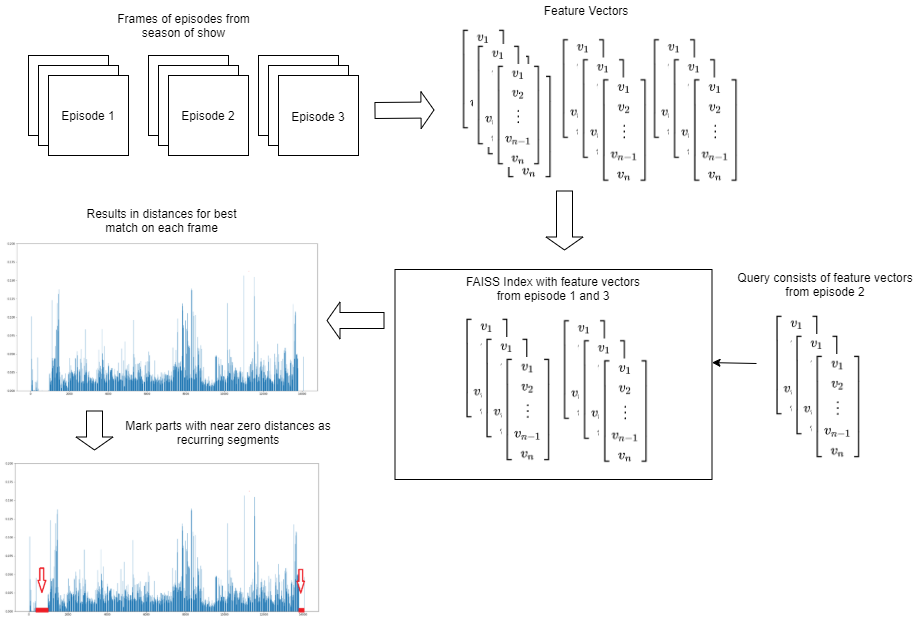
\includegraphics[width=\textwidth, center, scale=0.75]{images/thesisdiagram.png}
	\centering
	\caption{\textbf{Diagram of the described methodology. The recurring content detection process for episode 2 is portrayed.}}
	\label{fig:diagram}
\end{figure}

\subsection{Recurring Content}
To mark a part of the video as recurring content, we do the following steps: The frames of interest are converted to feature vectors while retaining the sequential order of episodes. Then the episode is used as an image query against all other episodes, resulting in a vector with distances for the best matches. We mark the locations of the indexes where these distances are lower than the percentile $p \in \{5\%, 7.5\%, 10\%\}$ of the lowest-distances vector. These are our initial detections. Because these detections can still contain noise, we do the following post-processing steps: Detections are merged into one if they are less than 10 seconds apart; and, we only keep the two largest detections within the first 20\% of the video or we keep the detection if it ends in the last 15 seconds of the video. The rationale behind this is that the recurring content that we want to detect is either in the first or last part of the video. See Figure \ref{fig:diagram} for a visual depiction of the described methodology.

\begin{algorithm}[H] 
	\SetAlgoLined
	
	import faiss
	
	percentile = 5 //or 7.5 or 10
	\texttt{\\}
	\texttt{\\}
	//Code for determining recurring content in episode with index i
	season = T\;
	episode = season.get(i)\;
	season.remove(i)\;
	episodeVectors = convertToVectors(episode)\;
	seasonVectors = convertToVectors(season)\;
	\texttt{\\}
	index = faiss.buildIndex(seasonVectors)\;
	distances = index.search(episodeVectors)\;
	\texttt{\\}
	threshold = getPercentileDistance(distances, percentile)\;
	\texttt{\\}
	recurringIndexes = new List()\;
	\For{i=0; i $<$ distances.length; i++}{
		distance = distances[i]\;
		\If{distance $<$ threshold }{
			recurringIndexes.add(i)\;
		}

	}
	\texttt{\\}
	//Merge indexes as recurring content when they are less than 10 seconds apart \\
	detections = MergeIndexes(recurringIndexes, 10)\;
	\texttt{\\}
	//Now only return the two largest detections in the beginning of the video \\
	//and detection that is at the end of a video \\
	detectionsAtStart = new List()\;
	detectionsAtEnd = new List()\;
	\For{i=0; i $<$ detections.length; i++}{
		detection = detections[i]\;
		\If{occursAtBeginOfVideo(detection) }{
			detectionsAtStart.add(detection)\;
		}
		\If{occursAtEndOfVideo(detection) }{
			detectionsAtEnd.add(detection)\;
		}
		
	}

	\textbf{return} getTwoLongestIntervals(detectionsAtStart) + detectionsAtEnd

	\caption{\textbf{Recurring content detection}}
	\label{algorithm:shotboundary}
\end{algorithm}

\subsection{Bumpers}
The methodology for detecting the bumpers within video content is different, because a bumper only contains recurring content from within the video itself. It shows shots that will be shown after the break, these shots may not reoccur in other episodes within a season. Therefore we cannot use the same methodology as described before for detection.

For the detection of bumpers we take a sliding window of 20 seconds of video frames, this will be the query. The index will consist of the remaining frames in the video, for every frame of interest the resulting distances of the two nearest neighbors will be saved and then this process is repeated for the next 20 seconds in the video all the way to the end.

After all the closest in-episode nearest neighbors are computed for each frame then from these results bumpers can be detected. We found that a global threshold for determining matches does not work well, probably because of the fact that bumpers are very short. Therefore we will use the ratio test described by Lowe \cite{lowe2004distinctive} for deciding on whether there is a match. With the ratio test the distance between the closest neighbor and second-closest neighbor is taken into account. The ratio of the distance of the closest neighbor to the distance of the second-closest neighbor determines whether there is a correct match, if the ratio is low then there is a higher chance for the match to be correct. In \cite{lowe2004distinctive} they classify a match to be correct if the ratio of the distances is equal to 0.8 or lower, we experimented with a ratio $r \in \{0.5, 0.6, 0.7, 0.8\}$ to find the optimal ratio for this problem.

\begin{algorithm}[H] 
	\SetAlgoLined
	
	import faiss\;
	RATIO = 0.5 // or 0.6 or 0.7 or 0.8 \\
	\texttt{\\}
	
	//Code for determining bumpers in episode with index i \\
	season = T\;
	episode = season.get(i)\;
	episodeVectors = convertToVectors(episode)\;
	\texttt{\\}
		
	//To get a stepsize of 10 seconds of video we need to jump (10*25)/3 indexes \\
	//because frames are subsampled every 3 frames \\
	stepSize = (10 * 25) / 3 \;
	currentStep = 0\;
	inEpisodeDistances = new List()\;
	\While{currentStep $<$ episodeVectors.size()}
	{
	\texttt{\\}
	 query = episodeVectors[currentStep:currentStep + stepSize] \;
	 index = faiss.buildIndex(EpisodeVectors[0:currentStep])\;
	 index.add(EpisodeVectors[currentStep+stepsize:episodeVectors.size()-1])\;
	 \texttt{\\}
	 //Compute 2 nearest neighbors for all frames in the current step \\
	 resultDistances = index.search(query, neighbors = 2)\;
	 inEpisodeDistances.concatenate(resultDistances)\;
	}

	ratios = inEpisodeDistances[:,0] / inEpisodeDistances[:,1]\;
	
	ratioIndexes = new List()\;
	\For{i=0; i $<$ ratios.length; i++}{
		ratios = ratios[i]\;
		\If{ratio $<$ RATIO }{
			ratioIndexes.add(i)\;
		}
		
	}
	
	//Return the consecutive ratio indexes  \\
	//that together are longer than 2.5 seconds \\
	return getConsecutiveRatioIndexes(ratioIndexes, 2.5)\;
	
	\caption{\textbf{Bumper detection}}
	\label{algorithm:shotboundary}
\end{algorithm}

\chapter{Results} \label{results}
This chapter contains the results for the experiments of detecting the recurring content (recaps, opening/closing credits and previews) and the experiments of the bumper detection.

\section{Recurring Content}
The results were evaluated as a retrieval problem. By doing so, the measures precision and recall could be used to describe the quality of recurring content detection for the methods proposed. Each second of recurring content is marked as a relevant instance and if recurring content gets detected, then those are relevant detected seconds, under this model we can calculate precision and recall as following:

\[\mathrm{precision} = \frac{\mathrm{detected\;relevant\;seconds}}{\mathrm{total\;detected\;seconds}}\]

\[\mathrm{recall} = \frac{\mathrm{detected\;relevant\;seconds}}{\mathrm{total\;relevant\;seconds}}\]

Because it is possible for the manual annotation to also be slightly inaccurate, we mark detections that are within a 2 second margin of the relevant section, to also be relevant. Figure \ref{fig:evaluation-example} depicts how the aforementioned precision and recall formulas apply to the detections and ground truth of a single episode. For the calculation of the total results on all episodes, the 'seconds' variables of all episodes are summed together and then precision and recall are calculated. The results are shown in Table \ref{table:resultsrecurring}. Plus the Precision-Recall curves for each recurring content class separately, in Figure \ref{fig:precision-recall}.

\begin{figure}[H]
	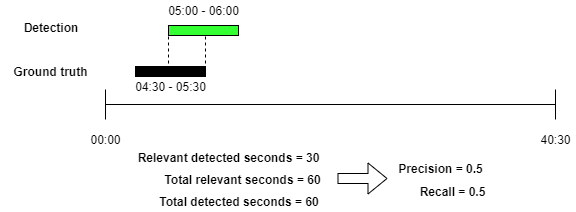
\includegraphics[width=\textwidth]{images/evaluation.png}
	\centering
	\caption{Visual example of the described evaluation methodology.}
	\label{fig:evaluation-example}
\end{figure}

\begin{table}[H]
	\begin{center}
		\begin{tabular}{ c c c c c c c} 
			\hline
			\textbf{Method} & \textbf{P} & \textbf{R} & \textbf{P} & \textbf{R} & \textbf{P} & \textbf{R} \\
			\hline
			\multicolumn{7}{c}{Uniform Sampling} \\
			 & \multicolumn{2}{c}{5\% lowest} & \multicolumn{2}{c}{7.5\% lowest} & \multicolumn{2}{c}{10\% lowest} \\
			\hline	
			CH 				& \textbf{0.884} 	& 0.687		& 0.830 	& 0.812 	& 0.786	 	& 0.855 \\
			CTM 			& 0.883 	& 0.681 		& 0.841 	& 0.796 & 0.796 	& 0.853 \\
			CNN 			& 0.854		& 0.733			& 0.808		& 0.838 & 0.748		& \textbf{0.892} \\
			\hline
			\multicolumn{7}{c}{Shotboundaries} \\
			\hline
			CH	 			& \textbf{0.904}		& 0.529 		& 0.852  	& 0.638 & 0.763	 	& 0.707 \\
			CTM 			& 0.856 	& 0.515 		& 0.830 	& 0.652 & 0.771		& \textbf{0.724} \\
			CNN 			& 0.837		& 0.522			& 0.800		& 0.635 & 0.725		& 0.713  \\
			\hline
		\end{tabular}
	\end{center}
	\caption{Results of the recurrent content detection at varying values for the lowest percentiles of distances.}
	\label{table:resultsrecurring}
\end{table}

\begin{figure}[h]
	\makebox[\textwidth][c]{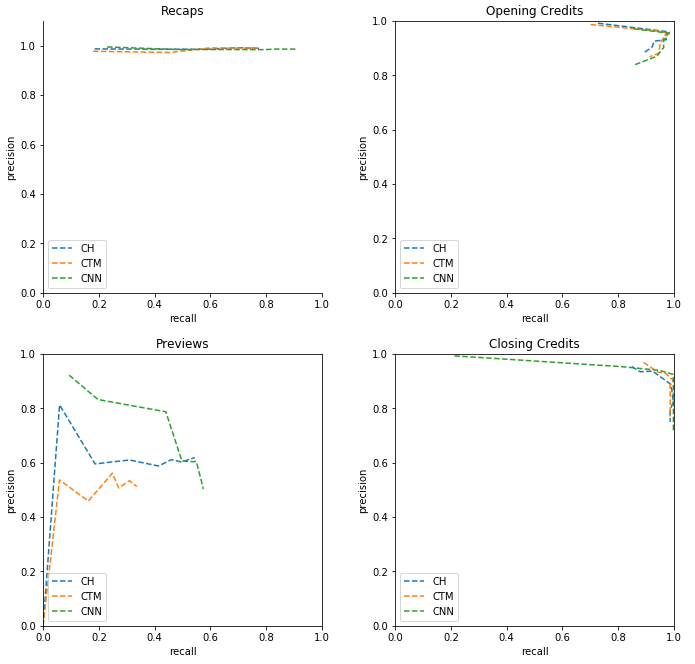
\includegraphics[scale=0.6]{images/precision-recall.png}}
	\centering
	\caption{Precision-Recall curves for each recurrent content class for the percentile values in the range [2.5, 20]. Data points that are in the upper right indicate good performance.}
	\label{fig:precision-recall}
\end{figure}

\section{Bumpers}
Because bumpers are short segments, the bumpers were evaluated in a different manner. We do not calculate precision and recall based on numbers of retrieved relevant seconds but consider only whether a detection has overlap with a bumper or not. If a detection has overlap with a bumper, then this detection is marked as relevant. Precision and recall will thus be calculated according to the following formulas:

\[\mathrm{precision} = \frac{\mathrm{detections\;with\;overlap}}{\mathrm{total\;detections}}\]

\[\mathrm{recall} = \frac{\mathrm{detections\;with\;overlap}}{\mathrm{total\;bumpers\;in\;episode}}\]

Figure \ref{fig:evaluation-example-bumpers} depicts how the precision and recall is calculated for the bumper detection. All the results of these experiments can be viewed in Table \ref{table:resultsbumpers}

\begin{figure}[H]
	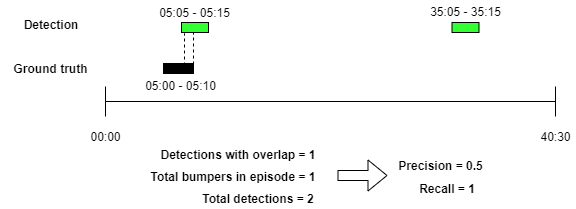
\includegraphics[width=\textwidth]{images/evaluation-bumpers.png}
	\centering
	\caption{Visual example of the described evaluation methodology for bumper detection.}
	\label{fig:evaluation-example-bumpers}
\end{figure}

\begin{table}[H]
	\begin{center}
		\begin{tabular}{ c c c c c c c c c} 
			\hline
			\textbf{Method} & \textbf{P} & \textbf{R} & \textbf{P} & \textbf{R} & \textbf{P} & \textbf{R} & \textbf{P} & \textbf{R} \\
			\hline
			& \multicolumn{2}{c}{\textbf{0.5 ratio}} & \multicolumn{2}{c}{\textbf{0.6 ratio}} & \multicolumn{2}{c}{\textbf{0.7 ratio}} & \multicolumn{2}{c}{\textbf{0.8 ratio}} \\
			\hline
			CH180 			& 0.195				& 0.312 		& 0.203		& 0.562		& 0.129		& 0.646 	& 0.085 	& 0.792 \\
			CTM 			&  0.145			& 0.542 		& 0.089		& 0.667 	& 0.072		& 0.833 	& 0.072 	& 0.958 \\
			CNN 			& \textbf{0.611}	& 0.917			& 0.484		& 0.938 	& 0.288		& \textbf{0.979} 	& 0.081 	& 0.979 \\
			\hline
		\end{tabular}
	\end{center}
	\caption{Results of the experiments on the bumper detection for varying values of the ratio test.}
	\label{table:resultsbumpers}
\end{table}

\section{Discussion} \label{discussion}
%interpretations
The results show that the performance of the different methods for recurrent segment detection, varying the feature vector construction approach, do not differ much. The way the feature vectors are constructed does not improve the results significantly when looking at the overall results. However, when looking at the scores for each class separately in Figure \ref{fig:precision-recall}, it can be noticed that the CNN-method performs better on the recaps and previews retrieval tasks. Possible explanations for this could be that the CNN-method is a local descriptor as opposed to a global one, therefore being able to handle the more tough cases of recaps and previews. Another explanation could be that higher dimensionality vectors are more suited, because the CNN vectors had the highest dimensionality.

Table \ref{table:resultsrecurring} presents that using shotboundaries results in lower recall scores compared to the uniform sampling of taking a frame every 3 frames. A possible explanation is that the shotboundary frames sometimes mismatch because the content shown does not consist of full shots.

Overall, the detection results are decent but not extraordinary, meaning that there is room for improvement in the methodology. 

The results of the different methods for the bumper detection show different performance results. The CNN-based method shows a large difference with the other methods. An explanation for this could be that again the CNN feature vectors are local descriptors as opposed to the other two methods that are global descriptors.

%limitations: what can't the results tell us
This thesis also does have its limitations. Most of the experiments are performed on the first three episodes of a single season. However, an end-solution would take a whole season into account. Also, sometimes the recurring content spans across different seasons (recapping the previous season in the first episode for example), our experiments did not take this attribute into account. We only took the visual data into account by looking at video frames, not utilizing the audio data. Future studies could incorporate audio data into the methodology to see if that improves the results.

The bumper detection is based on how RTL inserts its bumpers into content. With our experiments, we did not test if our methodology also applies to the bumpers of other publishers of commercial content.
\\
\iffalse
- I did not do an extensive study on all of the TV shows, so other edge cases are possible in other TV-shows.\\
- Very similar scenes occur regardless if it is a skippable segment or not\\
- Distances can be hard to navigate\\
- Using full seasons might give different results\\
- Video content is creative, never a clear structure, can encounter weird things (Changing of opening credit scenes, dismissal of opening credit scenes, rebroadcast of same content without it being a recap)\\
- Flash forwards/backwards confuse the model\\
- Recaps consisting of shot of different camera angles not used before

Future work: \\
- Take into account previous and next seasons\\
- Different methodologies for construction of the feature vectors\\
- Same methodology on different non-RTL data\\
- Take sound into account
\fi


\chapter{Conclusion and Future Work} \label{conclusion}
In this thesis we explored how well an image retrieval based approach could detect recurring content in a TV-show in an unsupervised manner. Experiments were performed using three different kind of feature vectors. Based upon these experiments we conclude that an image retrieval based approach definitely has potential for the unsupervised detection of recurrent content in TV-Shows. The experiments showed that the three different methods all get reasonable results. Overall, it is found that the CNN-based method using uniform frame sampling has the most potential. Using this method for a metadata labeling task will still require manual supervision. Future research is needed to improve upon the methodology or to experiment with other implementations of CNN-based feature vectors. This thesis presented novel research for the unexplored research area of recurring content detection that is focused on VOD content.

%recommendations: future studies
Future studies could be performed on a larger dataset consisting of full seasons of several shows to further prove the validity of this method and these future studies could try variations of the methodology and different ways of constructing the CNN feature vectors. Also the experiment could be repeated with data where the recurrent content classes are more in balance to verify the results.

%implications: why do the results matter
\iffalse
With these results we set the first steps towards a fully automated solution for detection of recurrent content. Much research has been done on broadcast streams, this thesis presents the first results on VOD content. Based on the results of the experiments it becomes clear that feature vectors constructed via a CNN have the most potential for the application to our problem.
\fi

\bibliographystyle{ieeetr}
\bibliography{references}

\end{document}
